\documentclass{article}%
\usepackage[T1]{fontenc}%
\usepackage[utf8]{inputenc}%
\usepackage{lmodern}%
\usepackage{textcomp}%
\usepackage{lastpage}%
\usepackage{authblk}%
\usepackage{graphicx}%
%
\title{Shox2 is a molecular determinant of depot{-}specific adipocyte function}%
\author{Alyssa Gutierrez}%
\affil{Department of Medicine, Addenbrooke's Hospital, University of Cambridge, Cambridge, United Kingdom}%
\date{01{-}01{-}2012}%
%
\begin{document}%
\normalsize%
\maketitle%
\section{Abstract}%
\label{sec:Abstract}%
UCLA researchers have shown that inflammation protects a specific type of a protein that protects against aging. The bifunctional enzyme found in fish is so effective against aging, the scientists found, that it remains active without food intake for 200 days after the body breaks down the protein and the cells break down the gene they believe is responsible for the proteins protection. Our findings explain a protein's role in the biology of aging, giving a new target for potential therapies, says lead author of the study, Rosalind Read, professor of molecular biology at the UCLA School of Medicine.\newline%
Read and her team had studied levels of the Protein Core Type I (PCI{-}I) on dystrophin{-}associated cells in the liver and kidneys and looked for evidence of any changes in these numbers before and after a drug was prescribed to treat the disease. The investigators worked with Dana Point{-}based Icos Corp., where Read is employed, to isolate and grow the central nervous system spheres of the NPC{-}I. They found that the protein circulates through these cells and appears to adhere to receptors on the cells where it binds the microbe known as dystrophin. Because the secretion mechanisms were slow and were derived from molecules associated with the human liver, spinal cord, kidney and brain, these cells served as a biological model for examining the effect of the injection of the drug in mice.\newline%
The conclusion drawn by the researchers is that the drug is able to bind a signal, called the butyrates of ethylglutamine, that is meant to fight the aging process. Read explains that the butyrates can also be studied because they replicate, knowing that DMI{-}I can activate them. The researchers believe that the drug interacts with other proteins that help support the function of the butyrates, so this makes it possible to study the role of additional proteins by looking at the peripheral blood.\newline%
The scientists hypothesize that over time, the butyrates will experience drug depletion as the NPC{-}I becomes older and likely needs to work to produce more of the proteins. In the body, this sort of dysfunctional signaling is associated with metabolic and metabolic diseases such as type 2 diabetes and cardiovascular disease. It is also an outcome of the misalignment of aging and metabolism. The UCSF Medical Center, in collaboration with Professor Read, first showed, in 2005, that dyes tied to a biological process called CD5+ was affecting chromosome 4 and CD8A in human livers.\newline%
Reads research was supported by Medical Science Council (CFST) grants, the California Institute for Regenerative Medicine (CIRM), the National Institute of Diabetes and Digestive and Kidney Diseases (CIRDM), the National Institutes of Health (NIH), New Jersey State Division of Diabetes Translation (NDSV), and the Swiss National Science Foundation. See:

%
\subsection{Image Analysis}%
\label{subsec:ImageAnalysis}%


\begin{figure}[h!]%
\centering%
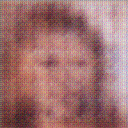
\includegraphics[width=150px]{500_fake_images/samples_5_352.png}%
\caption{A Close Up Of A Person Wearing A Tie}%
\end{figure}

%
\end{document}